\section{Von der Black Box „Internet“ und dem Wesen der Kommunikation}

\subsection{Vom Brief zur E-Mail}
Wenn man sich in früheren Jahrhunderten etwas Wichtiges und sehr Privates mitzuteilen hatte, traf man sich persönlich von Angesicht zu Angesicht. Wenn es die Distanz nicht erlaubte, musste man unter Umständen einen vertrauenswürdigen Boten engagieren, der die Nachricht in Form eines Briefes mit Siegel an die gewünschte Person überbrachte. Das Siegel sollte dabei die Integrität der im Brief enthaltenen Informationen gewährleisten. Was den zweiten Fall betraf, so hatte man auch da nicht die volle Kontrolle. Man musste wohl oder übel auf den Boten vertrauen. Hinzu kommt, dass dem Boten ja auch unterwegs etwas hätte zustossen können oder der Bote gezielt abgefangen wurde. Es gab also schon immer Unsicherheiten, was die Übertragung von Nachrichten betrifft, sofern man es nicht komplett selbst in die Hand nahm.
\\
Mit der Entwicklung des Postwesens, wie man es heute kennt, änderte sich vieles schlagartig. Briefe zu verschicken wurde bequem, einfach und bezahlbar. Jeder mit den nötigen Kleinutensilien konnte nun Briefe um die ganze Welt schicken - vorausgesetzt natürlich, man konnte schreiben. Wie sah es mit privaten bzw. geheimen Briefen aus? Erfahrungen aus der Vergangenheit, wie zum Beispiel die Postkontrollen zu STASI-Zeiten, haben gezeigt, dass es je nach Regierungsform der einzelnen Länder unterschiedlich sicher war, Privates per Post mitzuteilen. In den 80er Jahren wurden von der Abteilung M der STASI, welche für die Postkontrolle zuständig war, täglich bis zu 90 000 Briefe gelesen und/oder kontrolliert\footnote{Link 10, Linkverzeichnis, Briefmarkenverein Berliner Bär}.
Der Briefverkehr wird aber auch heute noch rege genutzt für aller Hand oberflächlicher Kommunikation und nicht selten auch für Privates. Wie kann man wissen, ob die Post nicht auch heute noch stellenweise kontrolliert wird?
\\
In den 70er-Jahren kam schliesslich das Internet und mit dem Internet das grosse Zeitalter der E-Mail. Die E-Mail war zu Beginn die meistgenutzte und wichtigste Anwendung des Internets und schon 1971 brauchte der E-Mail-Verkehr mehr Datenvolumen als alle anderen Dienste zusammen\footnote{Link 11, Linkverzeichnis, Wikipedia}
Nachrichten konnten nun noch günstiger - und vor allen Dingen schneller - übermittelt werden. Es gab zudem keine topographischen Einschränkungen, wenn die Infrastruktur einmal vorhanden war. Mailverkehr über das Internet hat viele Vorteile, das kann man nicht bestreiten. Er hat aber auch eine sehr grosse Schwachstelle. Das Internet ist heute in seiner Komplexität so enorm und vielschichtig, dass man als Laie kaum einschätzen kann, welchen Weg die verschickte E-Mail genau nimmt und welche Posten es dabei passiert.

\subsection{Der Webbrowser - Das Fenster zum Internet} 
Ein weiterer Meilenstein in der Geschichte des Internets ist der Webbrowser. Mit der Einführung des ersten grafikfähigen Webbrowsers Mosaic im Jahre 1993 erhielt das Internet einen weiteren Aufwärtsschub\footnote{Link 12, Linkverzeichnis, Wikipedia}.
Mit ihm war erstmals ein komfortables Durchstöbern des World Wide Web möglich, ganz ähnlich, wie man das heute mit bekannten Browsern wie dem Internet Explorer, Mozilla Firefox oder Google Chrome kann. Obwohl das Internet und das IT-Wesen allgemein immer komplexer und grösser werden, wird die oberflächliche Benutzung der Dienste immer einfacher. Surft man im Internet, um nach irgendwelchen Angeboten oder Online-Artikeln zu suchen, sieht man auf seinem Bildschirm lediglich ein Fenster, in dem man die gewünschten Inhalte in strukturierter und visuell aufbereiteter Form dargestellt bekommt. Woher die Daten genau kommen und welchen Weg sie nehmen ist nicht ersichtlich. Es ist eine Schnittstelle in ein riesiges Netzwerk von enormer Komplexität, die den Laien wohl sehr schnell überfordern würde. Und trotzdem ist die Bedienung kinderleicht.

\subsection{Die Cloud - Daten immer und überall}
Mit der passenden Software können heutzutage Daten immer und überall abgerufen werden. Beispielsweise werden Dokumente, die man auf verschiedenen Geräten braucht, regelmässig miteinander abgeglichen, um kein Durcheinander mit der Versionierung zu bekommen. Sie können sogar online bearbeitet werden, ohne beispielsweise ein Microsoft Office auf dem gerade genutzten PC installiert zu haben. Diese Möglichkeiten ergeben sich durch das immer stärker genutzte Konzept der \textit{Cloud}. Grosse IT-Unternehmen und Dienstleister mit der passenden Infrastruktur bieten dem Kunden eine Vielzahl von Diensten an, die alle über die Grossrechner der Unternehmen gehandhabt werden. Der Kunde hat dabei meist keine Einsicht in die technischen Einzelheiten und Prozesse und muss sich nicht mehr um technische Probleme kümmern. Er muss sich auch nicht fragen, wie denn eigentlich die Informationen von A nach B kommen und wo sie gespeichert werden. Für diesen Sachverhalt, der auch auf den E-Mail-Verkehr und das Surfen im Internet zutrifft, gibt es einen Fachbegriff. Man spricht von der sogenannten \textit{Black Box}.

\subsection{Das Prinzip der Black Box}
Der Begriff Black Box hat einen wissenschaftlichen Hintergrund. Die englischsprachige Seite von Wikipedia gibt folgende Kurzdefinition des Begriffes an:

\begin{quote}
\textit{A black box is a device, object, or system whose inner workings are unknown; only the input, transfer, and output are known characteristics}
\footnote{Link 13, Linkverzeichnis, Wikipedia}.
\end{quote}

Auf Deutsch übersetzt heisst das so viel wie: \textit{Eine Black Box ist ein Gerät, Objekt oder System, dessen innere Funktionsweise unbekannt ist. Nur die Eingabe, der Transfer und die Ausgabe sind bekannt.}
Man gibt also etwas in die Black Box hinein und erwartet einen bestimmten Output. Was genau in der Black Box vorgeht, wie der Output entsteht, interessiert einen nicht. Es zählt nur das Ergebnis. Eine einfache Grafik soll das Prinzip verdeutlichen.

\begin{figure}[H]
\centering
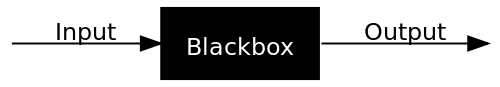
\includegraphics[scale=0.75]{images/BlackBox}
\caption{Black Box}
\end{figure}

Die drei Anwendungsfälle \textit{Mailverkehr},\textit{Surfen im Internet} und \textit{Nutzung der Cloud} machen ebenfalls von diesem Prinzip gebrauch. Möchte man einen Mailaccount einrichten, kann man dies gratis innerhalb weniger Minuten erledigen. Mails zu schreiben und anschliessend zu verschicken ist ebenfalls sehr komfortabel. Was das Surfen im Internet betrifft, so kann dies heute wohl jeder Zehnjährige. Das World Wide Web mit seinem riesen Fundus an Information ist zur Selbstverständlichkeit geworden. Lediglich der Gebrauch der Cloud ist für den Normalverbraucher noch nicht so selbstverständlich. Doch auch hier ist ein Trend zur vermehrten Verbreitung und Nutzung erkennbar. Im technischen Umfeld und in Unternehmen hat sich die Cloud schon längst durchgesetzt.
\\
\\
Es macht durchaus Sinn, dass man Dienste bewusst auslagert und konzentriert. Es kann schliesslich nicht jeder Mensch dieser Welt IT-Spezialist sein. Warum sollte man die technischen Fragen nicht denen überlassen, die sich in diesem Gebiet spezialisiert haben? Eine mögliche Antwort darauf gaben die letzten paar Monate, seit Edward Snowden die massenhafte und tiefgreifende Überwachung digitaler Medien durch diverse grosse Geheimdienste aufgedeckt hat. Die Überwachung betrifft auch den Mailverkehr, Daten bezüglich dem Surfverhalten der jeweiligen Nutzer und die Cloud-Dienste. Ähnlich wie früher beim Briefboten, legt man auch heute die Daten in die Hände von Dritten. Dies sind oft grosse, internationale Unternehmen, welche die Daten verarbeiten und aufbewahren. In die Einzelheiten des Verarbeitungsprozesses hat man dabei keinen Einblick. Es ist eine Black Box. Es war also bis heute alles eine Frage des Vertrauens und wird es vielleicht auch in Zukunft sein.
\\
\\
Die Enthüllungen Snowdens und die dadurch entstandenen Diskussionen zeigen aber eines ganz klar auf: Es braucht ein neues Bewusstsein, was das Internet, dessen Möglichkeiten,  Gefahren und die Privatsphäre betrifft. Die Frage des Datenschutzes ist einmal mehr in aller Munde und das zu Recht. Der gläserne Mensch - ein Mensch ohne Privatsphäre und Geheimnisse - scheint in greifbarer Nähe. Und ist er einmal Realität, lässt er sich nur schwer wieder verbannen
\footnote{Link 14, Linkverzeichnis, Wikipedia}.
\\
\\
Die Redewendung „Vertrauen ist gut, Kontrolle ist besser!“, die dem russischen Politiker Lenin zugeordnet wird
\footnote{Link 15, Linkverzeichnis, Wikipedia}, passt in diesem Zusammenhang ironischerweise sehr gut. Der Nutzer sollte mehr Kontrolle darüber haben, was mit seinen Daten passiert oder zumindest genau darüber Bescheid wissen. Es gibt dazu unterschiedliche Ansätze und sehr viele Möglichkeiten, diese Kontrolle zu erlangen. In den nächsten Kapiteln sollen ein paar davon gezeigt werden.

%Bilder:
%https://upload.wikimedia.org/wikipedia/commons/thumb/f/f6/Blackbox.svg/500px-Blackbox.svg.png
